%%%%%%%%%%%%%%%%%%%%%%%%%%%%%%%%%%%%%%%%%%%%%%%
\chapter{Computational Results} \label{chap:comp_method}
%%%%%%%%%%%%%%%%%%%%%%%%%%%%%%%%%%%%%%%%%%%%%%%

In Table \ref{tab:r_over_t}, our vector solutions are computed by
Algorithm \ref{alg:Increasing-Method} for the $\left(\epsilon=1,\ell=1\right)-\ensuremath{N}_{3,r,4}$
network regarding to $t=2$ and $t=3$, with $q_{v}=q^{t}$ as previous
sections. Both construction 1 and 2 provide better results than scalar
solutions. 

Construction 1: $\begin{array}{c|c}
\boldsymbol{I}_{t} & \boldsymbol{T}\end{array}$, with $\boldsymbol{T}\in\ensuremath{\mathbb{F}}_{q}^{t\times t\left(h-1\right)}$,
which is clearly explained in Section \ref{sec:Alternative-Approaches}.

Construction 2: $\boldsymbol{T}\in U\left(t,3t\right)$, which is
described in the following Section \ref{sec:Main-Approach}.

\section{Incremental Algorithm (IM) \label{sec:Main-Approach}}

Regarding to $t=2$, for a scalar network coding solution we need
a $3-\left(3,1,1\right)_{4}^{c}$ code ($q_{v}=2^{2}=4)$ by Theorem
\ref{theo:scalar_sol_exist}. The largest such code consists of the
21 one-dimensionall subspaces of $\ensuremath{\mathbb{F}}_{4}^{3}$,
each one is contained twice in the code. Therefore, the number of
nodes can be at most 42 for a scalar linear coding solution, while
for vector network coding 89 nodes can be used, i..e. $\mathcal{A}_{q=2}\left(n=6,k=4,\mathrm{t}=3;\lambda=2\right)\geq89$
following to Corollary \ref{cor:dual_subspaces}. This is a new lower
bound for $\mathcal{A}_{2}\left(6,4,3;2\right)$ compared to a code
with 51 codewords presented in \cite{Wachter-Zeh:2018}. The smallest
alphabet size for a scalar solution with 89 nodes exists is $q_{s}=8$.
By (\ref{eq:r_scalar_max}), there are 73 one-dimensional subspaces
of $\ensuremath{\mathbb{F}}_{8}^{3}$, and each one can be used twice
in the code; therefore, we have in total 146 possible codesword, but
only 89 codewords are required. In this case, the gap size $g=q_{s}-q_{v}=2^{3}-2^{2}=8-4=2^{2},$i.e.
we achieve a gap size $q^{t^{2}/2}$, which is better the asymptotic
behavior in (\ref{eq:gap_e1l1h3rs4}). 

Before introducing the algorithm used to generate such 89 codewords,
we have to state some definitions for a beter explanation. We denote
a matrix space of dimension $\left[n\times m\right]$ by $M(n,m)=\left\{ \boldsymbol{A}:\boldsymbol{A}\in\ensuremath{\mathbb{F}}_{q=2}^{n\times m}\right\} $.
\begin{defn}[Matrix Space with Unique Row Space\label{def:urs_matrix_space}]
 $U(n,m)$ is a subset of $M(n,m)$, where any $\boldsymbol{A},\boldsymbol{B}\in U(n,m)$
have their row spaces such that:
\[
\mathcal{R}_{q}\left(\boldsymbol{A}\right)\neq\mathcal{R}_{q}\left(\boldsymbol{B}\right),
\]
where $\mathcal{R}_{q}\left(.\right)$ denotes the row space of a
matrix.
\end{defn}
%
\begin{defn}[Sufficient Global Coding Vector\label{def:sufficient_global_coding_vectors} ]
 Let $\boldsymbol{A},\boldsymbol{B},\boldsymbol{C}\in U(t,3t)$ and
$N\lll\left(\begin{array}{c}
2^{3t^{2}}\\
3
\end{array}\right)$, then a set $\mathcal{H}_{n=3t,m=3t}=\left\{ \boldsymbol{H}_{1},\ldots,\boldsymbol{H}_{N}\right\} $
contains distinct \textit{sufficient global coding vectors} $\boldsymbol{H}_{j}$
such that:
\[
\mathrm{rk}\left[\boldsymbol{H}_{j}\right]=\mathrm{rk}\left[\begin{array}{c}
\boldsymbol{A}\\
\boldsymbol{B}\\
\boldsymbol{C}
\end{array}\right]\geq2n,\forall j\in\left\{ 1,\ldots,N\right\} .
\]
For ease of notations, we denote $\left[\begin{array}{c}
\boldsymbol{A}\\
\boldsymbol{B}\\
\boldsymbol{C}
\end{array}\right]$ by $\left\{ \boldsymbol{A},\boldsymbol{B},\boldsymbol{C}\right\} $
for the rest of this thesis.
\end{defn}
%
\begin{defn}[Relative]
 Let $\boldsymbol{A},\boldsymbol{B},\boldsymbol{C}\in U(t,3t)$ introduced
in Definition \ref{def:urs_matrix_space}. Then $\boldsymbol{C}$
is called a \textit{relative} of a tuple $\left(\boldsymbol{A},\boldsymbol{B}\right)$
if $\left\{ \boldsymbol{A},\boldsymbol{B},\boldsymbol{C}\right\} \in\mathcal{H}_{n=3t,m=3t}$
and denoted as following:
\[
\mathrm{rel}\left[\left(\boldsymbol{A},\boldsymbol{B}\right)\right]=\boldsymbol{C}.
\]
\end{defn}
\begin{lem}
For any set $\mathcal{H}_{n=3t,m=3t}=\left\{ \boldsymbol{H}_{1},\ldots,\boldsymbol{H}_{N}\right\} $,
there are maximum $3\cdot\left(\begin{array}{c}
2^{3t^{2}}\\
3
\end{array}\right)$ relatives. \label{lem:num_of_relatives}
\end{lem}
\begin{proof}
Each sufficient global coding vector $\boldsymbol{H}_{j}$ contains
a $\left\{ \boldsymbol{A},\boldsymbol{B},\boldsymbol{C}\right\} $.
Thus, each of these 3 matrices can form 3 different relatives:
\[
\begin{array}{c}
\mathrm{rel}\left[\left(\boldsymbol{A},\boldsymbol{B}\right)\right]=\boldsymbol{C}\\
\mathrm{rel}\left[\left(\boldsymbol{A},\boldsymbol{C}\right)\right]=\boldsymbol{B}\\
\mathrm{rel}\left[\left(\boldsymbol{B},\boldsymbol{D}\right)\right]=\boldsymbol{A}
\end{array}.
\]
Furthermore, the maximum size of $\mathcal{H}_{n=3t,m=3t}$ introduced
in Defnition \ref{def:sufficient_global_coding_vectors} is $q^{3t^{2}}$.
Therefore, $\mathcal{H}_{t=3}$ can have only maximum $3q^{3t^{2}}$
relatives.
\end{proof}
\begin{defn}[Sub-relative]
 Let $\boldsymbol{A},\boldsymbol{B},\boldsymbol{C},\boldsymbol{D}\in U(t,3t)$.
Then $\boldsymbol{D}$ is called a \textit{sub-relative} of a tuple
$\left(\boldsymbol{A},\boldsymbol{B},\boldsymbol{C}\right)\in\mathcal{H}_{n=3t,m=3t}$
if:
\[
\left\{ \begin{array}{c}
\left\{ \boldsymbol{A},\boldsymbol{B},\boldsymbol{D}\right\} \in\mathcal{H}_{t=3}\\
\left\{ \boldsymbol{A},\boldsymbol{C},\boldsymbol{D}\right\} \in\mathcal{H}_{t=3}\\
\left\{ \boldsymbol{B},\boldsymbol{C},\boldsymbol{D}\right\} \in\mathcal{H}_{t=3}
\end{array}\right..
\]
A sub-relative is denoted by: 
\[
\mathrm{subrel}\left[\left(\boldsymbol{A},\boldsymbol{B},\boldsymbol{C}\right)\right]=\boldsymbol{D}.
\]
This definition about Sub-relative is similarly again used for a set
of 5 or more matrices.
\end{defn}
\begin{algorithm}[H]
\caption{Increasing Method \label{alg:Increasing-Method}}

\hspace*{\algorithmicindent} \textbf{Input}: $\mathcal{H}_{n=3t,m=3t}$ with its size $\left|\mathcal{H}_{n=3t,m=3t}\right|=N\lll\left(\begin{array}{c} 2^{3t^{2}}\\ 3 \end{array}\right)$. \\
\hspace*{\algorithmicindent} \textbf{Output}: A $3-\left(3t,t,t\right)_{q=2}^{c}$ code or its orthogonal complement, a $3-\left(3t,2t,t\right)_{q=2}^{m}$ with its code size is maximum under $\mathcal{H}_{n=3t,m=3t}$.  
\begin{algorithmic}[1]
	\FORALL{$\left(\textbf{A},\textbf{B},\textbf{C}\right) \in \mathcal{H}_{n=3t,m=3t}$}
    	\STATE {$R\leftarrow$ Generate all relatives; ({*})}
	\ENDFOR

	\STATE {$P_{\mathrm{max}}\leftarrow\{\}$ // an empty set}
	\FORALL{$\left(\textbf{X},\textbf{Y}\right) \in R$} 
		\IF{$\left|\mathrm{rel}\left[\left(\textbf{X},\textbf{Y}\right)\right]\right|$ is maximum}
			\STATE {$P_{\mathrm{max}}\leftarrow P_{\mathrm{max}}\oplus\left(\textbf{X},\textbf{Y}\right)$ ({**})} 
		\ENDIF
	\ENDFOR

	\STATE {$P_{potential}\leftarrow\{\}$ // an empty set}
	\FORALL{$\left(\textbf{E},\textbf{Q}\right) \in P_{max}$}
		\IF{$\left|\left(\textbf{E},\textbf{Q}\right)\cup rel\left[\left(\textbf{E},\textbf{Q}\right)\right]\right|\notin P_{potential}$}
			\STATE {$P_{\mathrm{potential}}\leftarrow P_{\mathrm{potential}}\oplus\left(\textbf{E},\textbf{Q}\right)$}
		\ENDIF
	\ENDFOR
	
	\STATE {$P\leftarrow\{\}$ // an empty set}
	\FORALL{$\left(\textbf{K},\textbf{L}\right) \in P_{\mathrm{potential}}$}
		\FORALL{$\textbf{Z} \in \mathrm{rel}\left[\left(\textbf{X},\textbf{Y}\right)\right]$}
			\IF{$\mathrm{subrel}\left[\left(\boldsymbol{K},\boldsymbol{L},\boldsymbol{Z}\right)\right]$ is maximum}
				\STATE {$P\leftarrow P_{\mathrm{potential}}\oplus\left(\textbf{K},\textbf{L},\textbf{Z}\right)$ ({***})}
			\ENDIF
		\ENDFOR 
	\ENDFOR
	
	\WHILE{$\exists \mathrm{subrel}$ in $P$ is not empty ({****})}
		\STATE {Line 10 to Line 23, but elements of $P_{\mathrm{max}}$ is replaced by $P$ and the size of subrel tuple is thus increased over each while loop.}
	\ENDWHILE
\end{algorithmic}
\end{algorithm}

({*}): If any 2-tuple exists already in $R$, its new relative is
appended to its existing relatives to form a set of relatives.

({*}{*}): $P_{max}$ is set to an empty set anytime we find a new
maximum, before the concatenation $\oplus$.

({*}{*}{*}): $P$ is set to an empty set anytime we find a new maximum,
before the concatenation $\oplus$. $P$ removes duplicated values
itself under the while-loop of Line 11 to Line 15.

({*}{*}{*}{*}): This means the maximum size of subrel in $P$ is not
0.

~

Now, we prove that Algorithm \ref{alg:Increasing-Method} always give
us our expected output. Then we compute its complexity based on number
of necessary computation.
\begin{thm}
Let $n=\left|U(t,3t)\right|$, then the Algorithm \ref{alg:Increasing-Method}
finds all matrices satisfying Equation \ref{eq:rk_rqm_e1l1h3s4} for
the $\left(1,1\right)-\ensuremath{N}_{3,r,4}$ network in $\mathcal{O}\left(n^{3}\right)$
operations.
\end{thm}
\begin{proof}
Our problem can be described by searching for a matrix subset $\boldsymbol{c}=\left[\boldsymbol{C}_{1},\ldots,\boldsymbol{C}_{w}\right]$
of the set $U(t,3t)$ over $\ensuremath{\mathbb{F}}_{2}^{t\times3t}$
with $w\leq n$, such that any 3 matrices in $\boldsymbol{c}$ satisfy
Equation \ref{eq:rk_rqm_e1l1h3s4}. 

Line 1 to Line 3 (\textit{Step 1}) of the algorithm is for the purpose
of generating all relatives of pairs of 2 matrices in $U(2,6)$. With
a large $n$, we have $3\cdot\left(\begin{array}{c}
n\\
3
\end{array}\right)\approx3n^{3}$ such pairs for generating relatives. Outputs of this step are in
the format of 
\[
\mathrm{rel}\left[\left(\boldsymbol{C}_{i},\boldsymbol{C}_{j}\right)\right],\forall\left(\boldsymbol{C}_{i},\boldsymbol{C}_{j}\right)\in\mathrm{Combination}\left(U(2,6),2\right),
\]
where $\mathrm{Combination}(S,k)$ gives us all k-tuples of elements
in $S$. Let us denote the size of each $\mathrm{rel}\left[\left(\boldsymbol{C}_{i},\boldsymbol{C}_{j}\right)\right]$
by $m$, and we achive $3n^{3}$ different sizes in a vector $\boldsymbol{m}=\left[m_{1},\ldots,m_{3n^{3}}\right].$
Step 1 therefore can be implemented in $\mathcal{O}\left(n^{3}\right)$
operations. Following to Theorem \ref{theo:size_rel}, $\mathrm{max}\left\{ \boldsymbol{m}\right\} $
is the upper bound for a code size, when $3-\left(3t,t,t\right)_{q=2}^{c}$
code for a vector solution is considered \cite[Sec. V-D]{Zhang:2019}.

Line 4 to Line 9 (\textit{Step 2}) is designed to find all pairs $\left(\boldsymbol{C}_{i},\boldsymbol{C}_{j}\right)$
whose $m=max\left\{ \boldsymbol{m}\right\} $. This step ensures that
our output of the algorithm generate the largest size for the subset
$\boldsymbol{c}$, which is equivalent to an optimal vector solution
regarding to the use of $3-\left(3t,t,t\right)_{q=2}^{c}$ code. Step
2 checks all elements in $\boldsymbol{m}$, and thus it can be computed
in $\mathcal{O}\left(n^{3}\right)$ operations.

Line 10 to Line 15 (\textit{Step 3}) is designed to keep only one
of above intial pairs $\left(\boldsymbol{C}_{i},\boldsymbol{C}_{j}\right)$
if its set $\left\{ \boldsymbol{C}_{i},\boldsymbol{C}_{j}\right\} \cup\mathrm{rel}\left[\left(\boldsymbol{C}_{i},\boldsymbol{C}_{j}\right)\right]$
is duplicated with any other such pairs. Step 3 can be implemented
in $\mathcal{O}\left(n^{3}\right)$ operations.

Line 16 to Line 23 (\textit{Step 4}) is for the purpose of extending
a next matrix for this pair to form sub-relatives $\mathrm{subrel}\left[\left(\boldsymbol{C}_{i},\boldsymbol{C}_{j},\boldsymbol{C}_{p}\right)\right]$
by checking all relatives of each pair $\left(\boldsymbol{C}_{i},\boldsymbol{C}_{j}\right)$
from Step 3. We have $\mathrm{max}\left\{ \boldsymbol{m}\right\} \leq n-2$
because such a pair can have maximum $n-2$ relatives. Step 4 thus
can be computed in $\mathcal{O}\left(n\right)$ operations.

Line 24 to Line 26 (\textit{Step 5}): if there exist a non-empty set
$\mathrm{subrel}\left[\left(\boldsymbol{C}_{i},\boldsymbol{C}_{j},\boldsymbol{C}_{p}\right)\right]$
from outputs of Step 4. We run a loop of Step 3 and Step 4. This first
loop checks maximum $n-3$ elements, because such a triplet can have
maximum $n-3$. It will linearly reduce over each loop, and each loop
is designed to generate sub-relative, which costs maximum $\mathcal{O}\left(n\right)$
operations. Therefore, step 5 can be implemented in $\mathcal{O}\left(n^{2}\right)$
operations.

Summarized, we obtain the complexity claimed in the theorem.
\end{proof}
We are going to list some toy examples for the algorithm as well as
illustrate it in Figure \ref{fig:rel_example}.
\begin{example}
Let $n=1,m=2,q=2$, which violates the input $\mathcal{H}_{n=3t,m=3t}$
but still being a good example for the rest steps in Algorithm \ref{alg:Increasing-Method}.
Then we have $N=4$ matrices (vectors):
\[
\begin{array}{c}
\boldsymbol{A}=[0,0]\\
\boldsymbol{B}=[0,1]\\
\boldsymbol{C}=[1,0]\\
\boldsymbol{D}=[1,1]
\end{array}
\]
\uline{Step 1} (Line 1 to Line 3): Due to, any 3 of them form a
sufficient global coding vector, i.e. a matrix whose rank is greater
than or equal to $2n$, we have the relative as following:
\[
\begin{array}{c}
\mathrm{rel}\left[\left(\boldsymbol{A},\boldsymbol{B}\right)\right]=[\boldsymbol{C},\boldsymbol{D}]\\
\mathrm{rel}\left[\left(\boldsymbol{A},\boldsymbol{C}\right)\right]=[\boldsymbol{B},\boldsymbol{D}]\\
\mathrm{rel}\left[\left(\boldsymbol{A},\boldsymbol{D}\right)\right]=[\boldsymbol{B},\boldsymbol{C}]\\
\mathrm{rel}\left[\left(\boldsymbol{B},\boldsymbol{C}\right)\right]=[\boldsymbol{A},\boldsymbol{D}]\\
\mathrm{rel}\left[\left(\boldsymbol{B},\boldsymbol{D}\right)\right]=[\boldsymbol{A},\boldsymbol{C}]\\
\mathrm{rel}\left[\left(\boldsymbol{C},\boldsymbol{D}\right)\right]=[\boldsymbol{A},\boldsymbol{B}]
\end{array}
\]
\uline{Step 2} (Line 4 to Line 9): We get the maximum size of these
steps is $2$ and $P_{max}$ results in all $\left\{ \boldsymbol{A},\boldsymbol{B}\right\} ,\left\{ \boldsymbol{A},\boldsymbol{C}\right\} ,\left\{ \boldsymbol{A},\boldsymbol{D}\right\} ,\left\{ \boldsymbol{B},\boldsymbol{C}\right\} ,\left\{ \boldsymbol{B},\boldsymbol{D}\right\} ,\left\{ \boldsymbol{C},\boldsymbol{D}\right\} $,
since 
\[
\underset{\begin{array}{c}
\forall\boldsymbol{X},\boldsymbol{Y}\in M(1,2)\\
\boldsymbol{X}\neq\boldsymbol{Y}
\end{array}}{\mathrm{max}}\left(\mathrm{rel}\left[\left(\boldsymbol{X},\boldsymbol{Y}\right)\right]\right)=2
\]
.

\uline{Step 3} (Line 10 to Line 14): Due to $\left\{ \boldsymbol{E},\boldsymbol{Q}\right\} \cup rel\left[\left(\boldsymbol{E},\boldsymbol{Q}\right)\right]=\left\{ \boldsymbol{A},\boldsymbol{B},\boldsymbol{C},\boldsymbol{D}\right\} $
with $\left(\boldsymbol{E},\boldsymbol{Q}\right)$ are tuples from
$P_{max}$ found in Step 2. We keep only $P_{\mathrm{potential}}=\left\{ \left(\boldsymbol{A},\boldsymbol{B}\right):\mathrm{rel}\left[\left(\boldsymbol{A},\boldsymbol{B}\right)\right]\right\} $

\uline{Step 4} (Line 16 to 23): Regarding to $\mathrm{rel}\left[\left(\boldsymbol{K},\boldsymbol{L}\right)\right]=\mathrm{rel}\left[\left(\boldsymbol{A},\boldsymbol{B}\right)\right]$,
we have $\boldsymbol{Z}\in\left\{ \boldsymbol{C},\boldsymbol{D}\right\} $.
Then, $\left|\mathrm{subrel}\left[\left(\boldsymbol{A},\boldsymbol{B},\boldsymbol{C}\right)\right]\right|=\left|\mathrm{subrel}\left[\left(\boldsymbol{A},\boldsymbol{B},\boldsymbol{D}\right)\right]\right|=1$,
so we get $P=\left\{ \left(\boldsymbol{A},\boldsymbol{B},\boldsymbol{C}\right),\left(\left(\boldsymbol{A},\boldsymbol{B},\boldsymbol{D}\right)\right)\right\} $.

\uline{Step 5}: The maximum size of subrel in $P$ is larger than
$0$, so we proceed the while loop. Step 3 will be looped firstly,
and we get $P_{\mathrm{potential}}=\left\{ \left(\boldsymbol{A},\boldsymbol{B},\boldsymbol{C}\right):\mathrm{rel}\left[\left(\boldsymbol{A},\boldsymbol{B},\boldsymbol{C}\right)\right]\right\} $.

\uline{Step 6}: As step 4, we get a result $\left\{ \boldsymbol{A},\boldsymbol{B},\boldsymbol{C},\boldsymbol{D}\right\} $.
\end{example}
%
\begin{example}
For further understanding of Algorithm \ref{alg:Increasing-Method},
we use Figure \ref{fig:rel_example} for illustration. In Figure \ref{fig:rel_example}(c),
we observe that the size of relative becomes smaller when its tuple
identity is larger, i.e. $\left|\mathrm{rel}\left[\left(\boldsymbol{A},\boldsymbol{B}\right)\right]\right|\geq\left|\mathrm{subrel}\left[\left(\boldsymbol{A},\boldsymbol{B},\boldsymbol{C}\right)\right]\right|$
or $\left|\mathrm{rel}\left[\left(\boldsymbol{A},\boldsymbol{B}\right)\right]\right|\geq\left|\mathrm{subrel}\left[\left(\boldsymbol{A},\boldsymbol{B},\boldsymbol{D}\right)\right]\right|$.Regarding
to Figure \ref{fig:rel_example}(a) and \ref{fig:rel_example}(b),
the visual explanation of $\mathrm{subrel}$ is shown.
\end{example}
\begin{figure}[H]
\caption{An illustration of relatives and sub-relatives introduced in this
study for computational approaches of vector solutions for the $\left(\epsilon=1,\ell=1\right)-\ensuremath{N}_{h=3,r,s=4}$
network with $q^{t}=2^{2}$ and $q^{t}=2^{3}$ \label{fig:rel_example}}

\centering{}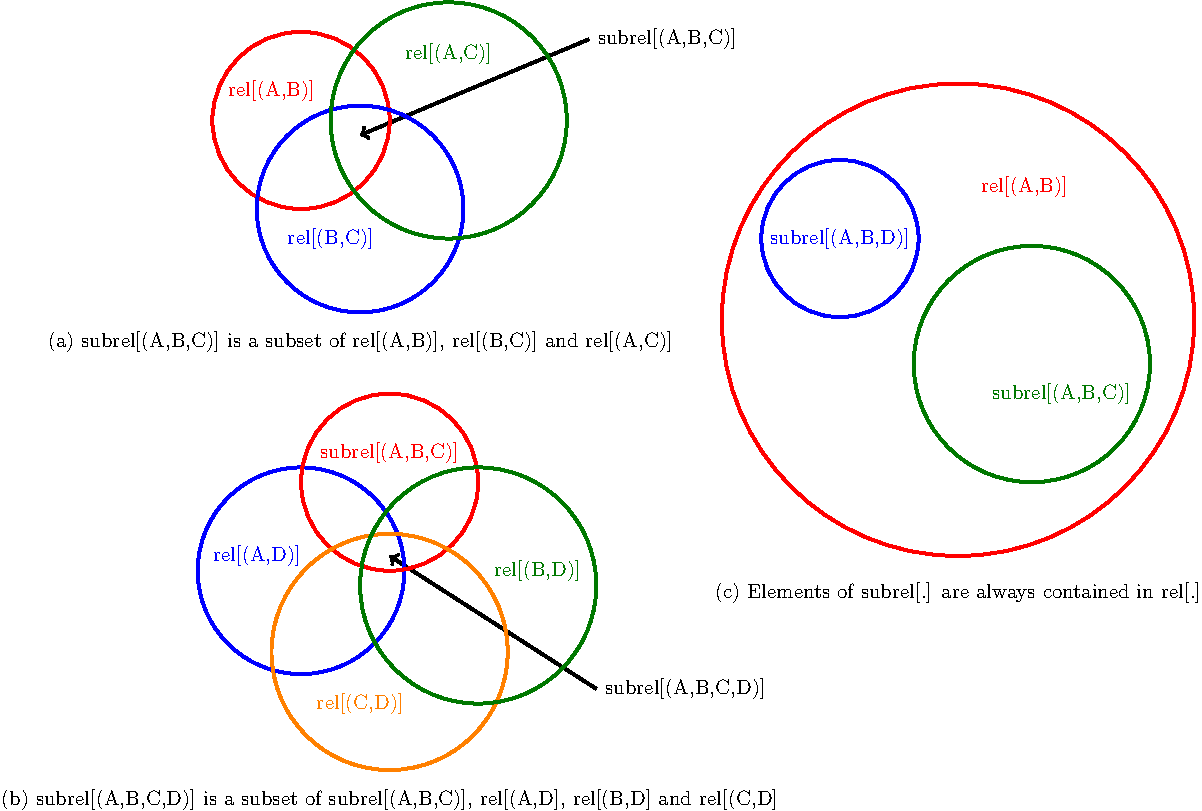
\includegraphics[width=0.5\paperwidth]{./figures/rel_example}
\end{figure}

\begin{thm}
The size of relatives and sub-relatives become smaller with there
are more elements in their identity tuples. \label{theo:size_rel}
\end{thm}
\begin{proof}
We call $\left(\boldsymbol{A},\boldsymbol{B}\right)$ of $\mathrm{rel}\left[\left(\boldsymbol{A},\boldsymbol{B}\right)\right]$,
$\left(\boldsymbol{A},\boldsymbol{B},\boldsymbol{C}\right)$ of $\mathrm{subrel}\left[\left(\boldsymbol{A},\boldsymbol{B},\boldsymbol{C}\right)\right]$,
or such $n$-tuples with $2\leq n\leq U\left(t,3t\right)$ by \textit{identity
tuples}. In Figure \ref{fig:rel_example}(a), we can see that 
\[
\mathrm{subrel}\left[\left(\boldsymbol{A},\boldsymbol{B},\boldsymbol{C}\right)\right]\in\left\{ \mathrm{rel}\left[\left(\boldsymbol{A},\boldsymbol{B}\right)\right]\cap\mathrm{rel}\left[\left(\boldsymbol{A},\boldsymbol{C}\right)\right]\cap\mathrm{rel}\left[\left(\boldsymbol{B},\boldsymbol{C}\right)\right]\right\} ,
\]

which gives us
\[
\begin{array}{c}
\mathrm{subrel}\left[\left(\boldsymbol{A},\boldsymbol{B},\boldsymbol{C}\right)\right]\subseteq\mathrm{rel}\left[\left(\boldsymbol{A},\boldsymbol{B}\right)\right],\\
\mathrm{subrel}\left[\left(\boldsymbol{A},\boldsymbol{B},\boldsymbol{C}\right)\right]\subseteq\mathrm{rel}\left[\left(\boldsymbol{A},\boldsymbol{C}\right)\right],\\
\mathrm{subrel}\left[\left(\boldsymbol{A},\boldsymbol{B},\boldsymbol{C}\right)\right]\subseteq\mathrm{rel}\left[\left(\boldsymbol{B},\boldsymbol{C}\right)\right].
\end{array}
\]
Therefore,
\[
\left|\mathrm{rel}\left[\left(\boldsymbol{A},\boldsymbol{B}\right)\right]\right|\geq\left|\mathrm{subrel}\left[\left(\boldsymbol{A},\boldsymbol{B},\boldsymbol{C}\right)\right]\right|,
\]
which is still true when the size of identity tuples becomes smaller.
\end{proof}
We have tried 2 variants of the above algorithm as following. Firstly,
instead of using \textit{matrix space with unique row space}, we use
the whole matrix space $M\left(n,m\right)$ introduced in Definition
\ref{def:urs_matrix_space}. In case $t=2$, we cover all $2^{3t^{2}}=4096$
matrices instead of only 715 matrices in Section \ref{sec:Main-Approach},
which will help the Algorithm \ref{alg:Increasing-Method} cover the
optimal vector solution.
\begin{defn}[Good Global Coding Vector\label{def:almost_sufficient_global_coding_vector}]
 Let $\boldsymbol{A},\boldsymbol{B},\boldsymbol{C}\in U(t,3t)$ and
$N\leq\left(\begin{array}{c}
2^{3t^{2}}\\
3
\end{array}\right)$, then a set $\mathcal{T}_{n=3t,m=3t}=\left\{ \boldsymbol{T}_{1},\ldots,\boldsymbol{T}_{N}\right\} $
contains distinct \textit{sufficient global coding vectors} $\boldsymbol{T}_{j}$
such that:
\[
\mathrm{rk}\left[\boldsymbol{T}_{j}\right]=\mathrm{rk}\left[\begin{array}{c}
\boldsymbol{A}\\
\boldsymbol{B}\\
\boldsymbol{C}
\end{array}\right]\geq2n,\forall j\in\left\{ 1,\ldots,N\right\} .
\]
In Algorithm \ref{alg:Increasing-Method}, we substitute the input
by $\mathcal{T}_{n=3t,m=3t}$ instead of $\mathcal{H}_{n=3t,m=3t}$.
This will give us an output with upper bound of $\mathcal{A}_{2}\left(3t,2t,3;2t\right)=126$
\cite[Sec. V-B]{Zhang:2019}. We can see that $\left|\mathcal{T}_{n=3t,m=3t}\right|\approx11\cdot10^{9}\gg\left|\mathcal{H}_{n=3t,m=3t}\right|\approx60\cdot10^{6}$.
\end{defn}
Secondly, we tried another approach called ``Randomly Increasing
Method''. We got about 72 codewords instead of 89 codewords as Algorithm
\ref{alg:Increasing-Method}, due to a limited number of tries. Briefly,
this approach started with a pair of the following 2 potential matrices
\[
\left[\begin{array}{cccccc}
0 & 0 & 0 & 0 & 0 & 0\\
0 & 0 & 0 & 0 & 0 & 0
\end{array}\right],\left[\begin{array}{cccccc}
1 & 0 & 0 & 0 & 0 & 0\\
0 & 1 & 0 & 0 & 0 & 0
\end{array}\right].
\]
Then we tried adding a new random matrix from $U\left(t=2,3t=6\right)$
into a list containing this pair. The random matrix is extended to
the list, if the matrix and any 2 existing matrices in the list satisfy
(\ref{eq:rk_rqm_e1l1h3s4}). The list will be extended until all matrices
in $U\left(t=2,3t=6\right)$ are checked.

\section{Decremental Algorithm (DM) \label{sec:Alternative-Approaches}}

In Algorithm \ref{alg:Decreasing-Method}, we introduce a decremental
algorithm by removing bad matrices from a set of 715 matrices, until
any 3 of the matrices left in the set satisfy (\ref{eq:rk_rqm_e1l1h3s4}).
A matrix with the less number of occurence in $\mathcal{T}_{n=3t,m=3t}$
or $\mathcal{H}_{n=3t,m=3t}$ is evaluated as a bad matrix, and it
is removed for each step. If many bad matrices exist, we only remove
the first one, which makes this algorithm a random one and require
multiple tries. In case $t=2$, we tried once with $\left|U\left(t,3t\right)\right|=715$
matrices as the algorithm's input, and unfortunately got about 69
codewords instead of 89 codewords as Algorithm \ref{alg:Increasing-Method}. 

\begin{algorithm}[H]
\caption{Decreasing Method \label{alg:Decreasing-Method}}

\hspace*{\algorithmicindent} \textbf{Input}: $U(t,3t)$. \\
\hspace*{\algorithmicindent} \textbf{Output}: A subset of $U(t,3t)$ with any 3 matrices satisfy Equation \ref{eq:p_in_LLL}. 
\begin{algorithmic}[1]
	\STATE {$\left[\textbf{L}_{0},\ldots,\boldsymbol{L}_{\left|U(t,3t)\right|-1}\right]\leftarrow U(t,3t)$ // Assign all matrices into a list.}
	\STATE {$\boldsymbol{j}\leftarrow\left[\boldsymbol{L}_{0},\ldots,\boldsymbol{L}_{\left|U(t,3t)\right|-1}\right]$}
	\REPEAT
	\STATE {$\boldsymbol{g}\leftarrow\left[0,\ldots,0\right]$ with $\left|\boldsymbol{g}\right|=\left|\boldsymbol{j}\right|$ // Number of occurences for bad matrices}
	\FORALL{$\left[c_{0},c_{1},c_{2}\right]\in\left(\begin{array}{c} \left|\boldsymbol{j}\right|\\ 3 \end{array}\right)$}
		\IF{$rk\left[\begin{array}{c} \boldsymbol{j}_{c_{0}}\\ \boldsymbol{j}_{c_{1}}\\ \boldsymbol{j}_{c_{2}} \end{array}\right]\leq2t$}	
			\STATE {$\textbf{g}_{c_{0}}\leftarrow \textbf{g}_{c_{0}}+1$}
			\STATE {$\textbf{g}_{c_{1}}\leftarrow \textbf{g}_{c_{1}}+1$}
			\STATE {$\textbf{g}_{c_{2}}\leftarrow \textbf{g}_{c_{2}}+1$}
		\ENDIF
	\ENDFOR
	\STATE {remove $\boldsymbol{j}_{max\left[\boldsymbol{g}\right]\neq0}$ from $\boldsymbol{j}$}
	\UNTIL{$max\left[\boldsymbol{g}\right]=0$}
\end{algorithmic}
\end{algorithm}
Finally, construction 1 mentioned in Section \ref{sec:Main-Approach}
to achieve a vector solution for the $\left(1,1\right)-\mathcal{N}_{3,r,4}$
network with $t=3$, which has not been yet found in any other papers.
When $t=3$, a $3-\left(9,3,3\right)_{4}^{c}$ code is required for
a vector solution of the network by Theorem \ref{theo:scalar_sol_exist}.
Its orthogonal complement is a $3-\left(9,6,2\right)_{q}^{m}$ code,
and the bound for this code is denoted by $\mathcal{A}_{2}\left(9,6,3;2\right)$
following to Corollary \ref{cor:dual_subspaces}. In \cite{Etzion:2018},
they only covered $\mathcal{A}_{2}\left(6,k,t;2\right),\mathcal{A}_{2}\left(7,k,t;2\right)$,
and $\mathcal{A}_{2}\left(8,k,t;2\right)$, this is thus a newly found
bound for a vector solution of the $\left(1,1\right)-\mathcal{N}_{3,r,4}$
network. We listed 166 three-dimensional subspaces of $\ensuremath{\mathbb{F}}_{2}^{9}$
in Appendix \ref{sec:166-Three-Dimensional-Subspaces}. Therefore,
we conclude $166\leq\mathcal{A}_{2}\left(9,6,3;2\right)$. By Theorem
\ref{theo:zhang-theorem10}, we achieve its upper bound $\mathcal{A}_{2}\left(9,6,3;2\right)\leq1129$.
The upper bound can be improved by Theorem \ref{theo:zhang-theorem11}
with $\mathcal{A}_{2}\left(9,6,3;2\right)\leq\left\lfloor \frac{85}{21}\mathcal{A}_{2}\left(8,5,2;2\right)\right\rfloor \leq537$,
where $33\leq\mathcal{A}_{2}\left(8,5,2;2\right)\leq128$ in \cite[Table 3]{Etzion:2018}.
Hence, we have $166\leq\mathcal{A}_{2}\left(9,6,3;2\right)\leq537$.
\begin{thm}[{\cite[Theorem 10]{Zhang:2019}\label{theo:zhang-theorem10}}]
 If $n,k,\mathrm{t}$ and $\lambda$ are positive integers such that
$1\leq\mathrm{t}<k<n$ and $1\leq\lambda\leq\left[\begin{array}{c}
n-\mathrm{t}\\
k-\mathrm{t}
\end{array}\right]_{q}$, then,
\[
\mathcal{A}_{q}\left(n,k,\mathrm{t};\lambda\right)\leq\left\lfloor \lambda\frac{\left[\begin{array}{c}
n\\
\mathrm{t}
\end{array}\right]_{q}}{\left[\begin{array}{c}
k\\
\mathrm{t}
\end{array}\right]_{q}}\right\rfloor 
\]
\end{thm}
%
\begin{thm}[{\cite[Theorem 11]{Zhang:2019}\label{theo:zhang-theorem11}}]
 If $n,k,\mathrm{t}$ and $\lambda$ are positive integers such that
$1\leq\mathrm{t}<k<n$ and $1\leq\lambda\leq\left[\begin{array}{c}
n-\mathrm{t}\\
k-\mathrm{t}
\end{array}\right]_{q}$, then,
\[
\mathcal{A}_{q}\left(n,k,\mathrm{t};\lambda\right)\leq\left\lfloor \frac{q^{n}-1}{q^{k}-1}\mathcal{A}_{q}\left(n-1,k-1,\mathrm{t}-1;\lambda\right)\right\rfloor 
\]

\newpage{}
\end{thm}
\begin{sidewaystable}[H]
\begin{centering}
\begin{tabular}{|c|c|c|c|c|c|}
\hline 
t & Scalar Solution ({*}) & Vector Solution ({*}) & Etzion and Kurz & Construction 1 (IM) & Construction 2 (IM)\tabularnewline
\hline 
\hline 
2 & $r_{\mathrm{max,scalar}}=42$ & $r_{\mathrm{max,vector}}\geq7$ & $r_{\mathrm{max,vector}}=121$ & $r_{\mathrm{max,vector}}=89$ & N/A\tabularnewline
\hline 
3 & $r_{\mathrm{max,scalar}}=146$ & $r_{\mathrm{max,vector}}\geq62$  & N/A & N/A & $r_{\mathrm{max,vector}}=166$\tabularnewline
\hline 
4 & $r_{\mathrm{max,scalar}}=546$ & $r_{\mathrm{max,vector}}\geq1317$ & N/A & N/A & N/A\tabularnewline
\hline 
5 & $r_{\mathrm{max,scalar}}=2114$ & $r_{\mathrm{max,vector}}\geq58472$ & N/A & N/A & N/A\tabularnewline
\hline 
6 & $r_{\mathrm{max,scalar}}=8322$ & $r_{\mathrm{max,vector}}>10^{6}$ & N/A & N/A & N/A\tabularnewline
\hline 
\end{tabular}
\par\end{centering}
\centering{}\caption{Vector solutions outperform the optimal scalar solution for the $\left(\epsilon=1,\ell=1\right)-\mathcal{N}_{h=3,r,s=4}$
network over $t=2,\ldots,6$. For $t=2$, the vector solution found
in \cite{Etzion:2018} gives the largest number of the intermediate
nodes with $r_{\mathrm{max,vector}}=121$. For $t=3$, our vector
solution gives a better result than both the optimal scalar solution
and the combinatorial vector solution with $r_{\mathrm{max,vector}}=166$.
For $t=3,\ldots,6$, all of our combinatorial vector solutions outperform
the optimal scalar one. ({*}): combinatorial results based on Table
\ref{tab:r_over_t}.\label{tab:r_over_t-1}}
\end{sidewaystable}

\clearpage